% vim: set spell:
% vim: set spell spelllang=en:
\documentclass[a4paper,10pt]{article}
%\usepackage[mathjax]{lwarp}
%\usepackage{lwarp}
\usepackage[utf8]{inputenc}
\usepackage{tikz}
\usepackage[T1]{fontenc}
\usepackage{amsfonts}
\usepackage{amsmath}
\usepackage{pifont}
\usepackage{tikz}
\usetikzlibrary{calc}
\usepackage{hyperref}
\usepackage{stmaryrd}
\usepackage[left=2cm,right=2cm]{geometry}

\title{Tutorials : Concepts of Logic and Programming}
\author{Nicolas González}
\date{September 25th 2020}

\def\centralruler{\begin{center}\rule{5cm}{.1pt}\end{center}}

\newcommand{\R}{\mathbb{R}}
\newcommand{\Com}{\mathbb{C}}
\newcommand{\K}{\mathbb{K}}
\newcommand{\Z}{\mathbb{Z}}
\newcommand{\N}{\mathbb{N}}
\newcommand{\Lin}{\mathcal{L}}
\newcommand{\Mnn}{\mathcal{M}_n(\R)}
\newcommand{\ProScal}[2]{\langle #1,#2 \rangle}
\newcommand{\Norm}[1]{\left|\left| #1 \right|\right|}
\newcommand{\grad}{\overrightarrow{\nabla}}
\newcommand{\Proba}{\mathbb{P}}
\newcommand{\vv}[1]{\overrightarrow{\textbf{#1}}}

\DeclareMathOperator{\Vect}{Vect}
\DeclareMathOperator{\Imag}{\Im m}
\DeclareMathOperator{\Mat}{Mat}
\DeclareMathOperator{\rk}{rk}
\DeclareMathOperator{\asinh}{asinh}


\renewcommand{\theequation}{\thesubsection--\arabic{equation}}


\newcommand{\Tstrut}{\rule{0pt}{2.6ex}}
\newcommand{\Bstrut}{\rule[-0.9ex]{0pt}{0pt}}
\newcommand{\TBstrut}{\Tstrut\Bstrut}
%\usepackage[toc]{glossaries}
%\makeglossaries
%\loadglsentries{glossary}

\begin{document}

\maketitle
%\tableofcontents

\newpage

\section{Exercise 1 : Bascules}
\begin{enumerate}
	\item Réaliser les bascules RS et JK à l'aide d'une bascule D et de portes
	\item Réaliser la bascule D à l'aide d'une bascule T et de portes
	\item Réaliser les bascules D et T à l'aide d'une bascule JK et de portes
\end{enumerate}
\centralruler

It's all in the logisim files!

\section{Exercise 2}
On considère l'assemblage synchrone suivant (synchronisé par une seule horloge) :
\begin{center}
	\includegraphics[scale=.6]{machine_3_2.png}
\end{center}

\begin{enumerate}
	\item Donner la table des états et le diagramme des états de la fonction de sortie fs et de la fonction de transition ft.
	\item Dessiner le diagramme temporel pour la séquence 01101 présentée sur l'entrée R.
\end{enumerate}

\centralruler

\subsection{Question 1}

Let's begin with state tables. Those tables list the input and the internal state of the machine and the values for the transition and output functions.

Let's try and understand these two notions first. In our machine, which is a Moore machine (since the input does not directly influence the output).

So the transition function is the combination of our two and gates, because that is what will influence the new state. Our state is the combination of the two bits stored in both D flip flops.

Our output function is the identity of the state : each output has a corresponding flip flop it directly mirrors.

Let's write our state table.
\begin{center}
	\begin{tabular}{|c|c|c|c|}
		\hline
		$R$&$(S_2,S_1)$&$f_t(R,(S_2,S_1))$&$f_s(R,(S_2,S_1))$\\\hline
		$0$&$00$&$00$&$00$\\\hline
		$1$&$00$&$01$&$01$\\\hline
		$0$&$01$&$00$&$00$\\\hline
		$1$&$01$&$11$&$11$\\\hline
		$0$&$10$&$00$&$00$\\\hline
		$0$&$11$&$00$&$00$\\\hline
		$1$&$11$&$11$&$11$\\\hline
	\end{tabular}
\end{center}

As for the state diagram, each bubble shows the current state, and the arrows are adorned with the input, a slash, and the corresponding output. We get the figure shown here.

\begin{figure}[ht]
	\centering
	% I'm sorry
	\includegraphics[scale=.8]{ex_3_2_state_diagram.png}
\end{figure}

\subsection{Question 2}

As for the time based diagram, for the sake of convenience, and because everything changes at the same moment every clock top, I will use a table.

\begin{table}[ht]
	\centering
	\begin{tabular}{|c|c|c|c|c|c|}
	\hline
	Label&Top 1&Top 2&Top 3&Top 4&Top 5\\\hline
	H (clock down omitted)&1&1&1&1&1\\\hline
	R&0&1&1&0&1\\\hline
	S1&0&1&1&0&1\\\hline
	S2&0&0&1&1&0\\\hline
	\end{tabular}
\end{table}

\section{Exercise 3 : détecteur de transitions positives}

Réaliser un détecteur de transitions positives ou négatives. L'entrée $e$ vaut $0$ ou $1$ pendant des cycles entiers. Les sorties $s1$ (passage de $0$ à $1$) et $s2$ (passage de $1$ à $0$) doivent valoir $1$ pendant le cycle qui suit la transition.
\begin{enumerate}
	\item Décrire un diagramme des états pour ce circuit
	\item Réaliser ce circuit à l'aide de bascules $D$.
\end{enumerate}

\centralruler

\subsection{Question 1}

I hate doing state diagrams because I can't draw them easily in LaTeX, but oh well.
Essentially our machine has one input, and one internal state (that keeps track of what the former value of the input was ; let's call it $I$). Both of those should trigger an output (this is a Mealy machine) when they differ, but they should be controlled to know which output is triggered.

Let's list our states :
\begin{enumerate}
	\item The previous input was 0
	\item The previous input was 1
\end{enumerate}

The spoiler here is that we need two bits of internal memory. Let's call it $(I,J)$ with our previous notation, we get
\begin{figure}[ht]
	\centering
	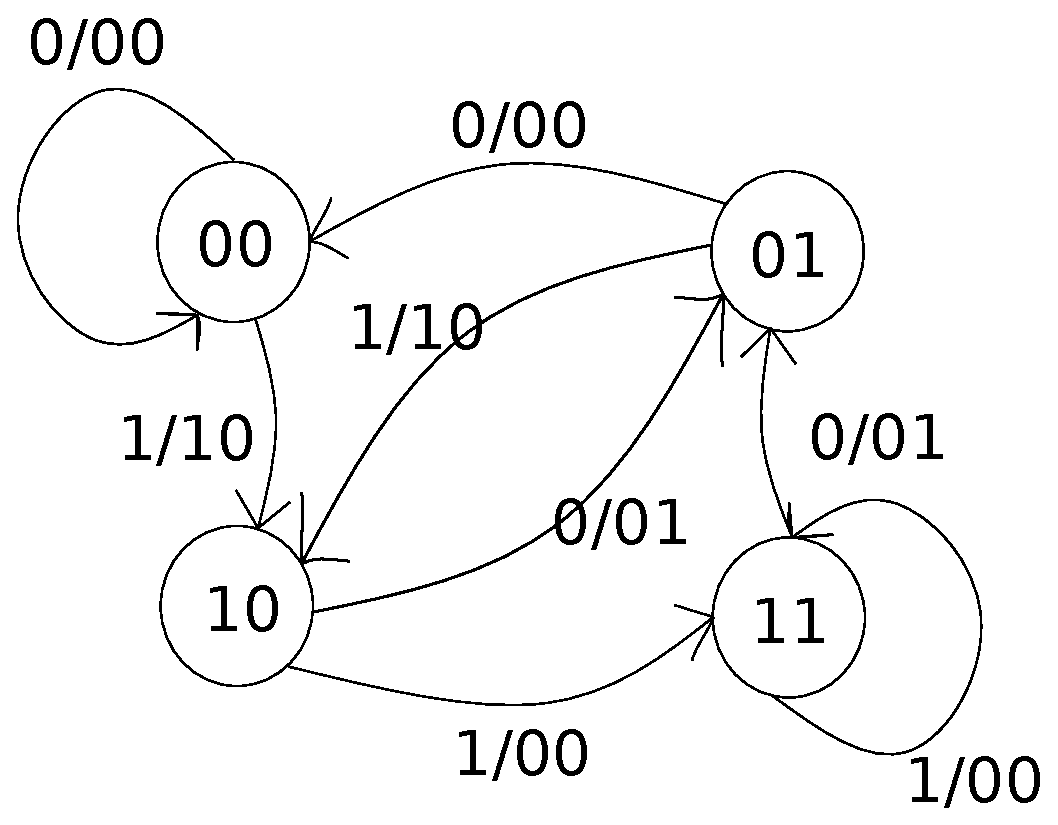
\includegraphics[scale=.4]{ex_3_3.eps}
	\caption{State Diagram for the Machine}
\end{figure}

If we use $(s_1,s_2)$ as our output tuple in this diagram, we can see that when we stay in the same state, none of them light up. When we flip from state $I=1$ to $I=0$ we need to light $s2$ on, and when we go the other way around we light $s1$ on.

But there's a catch, it needs to happen one tick late, so we need to store in memory the state of that tick having happened, and then output what we should, and we're good.

\subsection{Question 2}
Here's the implementation in logisim (in the file given alongside this pdf).

\begin{figure}[ht!]
	\centering
	\includegraphics[scale=.6]{machine_3_3.png}
\end{figure}

\section{Exercise 4 : ``est divisible ou non par cinq''}

On désire réaliser un circuit qui détermine si un nombre, reçu bit à bit en commençant par les bits de poids forts, est divisible ou non par cinq.

La sortie $Est_div$ indique si le nombre constitué de la suite des bits reçus sur $Nbre$ depuis le dernier $Init$ est divisible par $cinq$. Le premier bit du nombre est reçu dans le cycle qui suit la commande $Init$. On note $R(N)$ le reste de la division d'un nombre $N$ par $5$.
\begin{enumerate}
	\item Indiquer par une table la valeur des restes $R(2N)$ et $R(2N+1)$ en fonction de $R(N)$.
	\item En déduire le diagramme des états du circuit.
	\item Donner un schéma de réalisation.
\end{enumerate}

\centralruler

\subsection{Question 1}

There are only five possible remainder values $R(N)$ which are $0$, $1$, $2$, $3$ and $4$. For example, if a number is $a=2\times n$ with $n\in\N$, then $2a=2*n*5$ and both will have a remainder of $0$. When $a=5n+1$, then $2a=10n+2$, and so on (i.e. the remainder is multiplied by two and obtained modulo five). As for $R(2N+1)$, the computations are the same ($a=2n\implies(2a+1)=10n+1$ so $1$ for the remainder and so on).

We find the following table
\begin{table}[ht!]
	\centering
	\begin{tabular}{|c|c|c|}
		\hline
		$R(N)$&$R(2N)$&$R(2N+1)$\\\hline
		$0$&$0$&$1$\\\hline
		$1$&$2$&$3$\\\hline
		$2$&$4$&$0$\\\hline
		$3$&$1$&$2$\\\hline
		$4$&$3$&$4$\\\hline
	\end{tabular}
\end{table}

\subsection{Question 2}

This technique is very smart since pushing a $0$ into the input is like multiplying $N$ by $2$, and pushing a $1$ is just $2\times N+1$, and since $0$ is divisible by $5$, we can just travel along a given amount of states.

We need to store enough information to remember the remainder, so 3 bits (8 possible values, only 5 of which we'll need). Let's call them $(s3,s2,s1)$. We keep jumping value depending on whether we add a $0$ or a $1$ to the input, and of course the init is also taken into account (so let's write it $(init,nbre)$). We find

\begin{figure}[ht!]
	\centering
	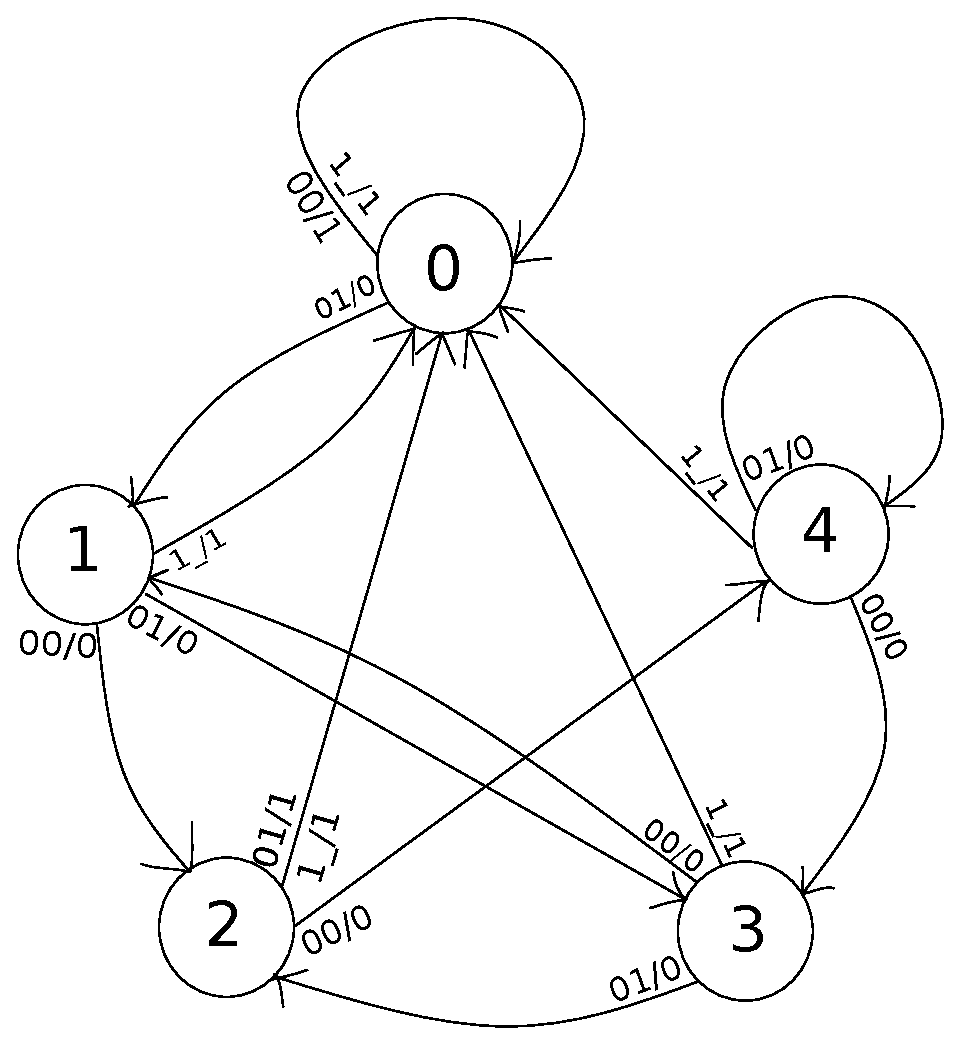
\includegraphics[scale=.7]{ex_3_4.eps}
	\caption{Machine state diagram for exercise 3.4}
\end{figure}

Almost satanic isn't it? The circuit is worse.

\subsection{Question 3}

Here's a screenshot of the circuit. It uses 3 flip flops to remember the information $(s3,s2,s1)$ and computes its new state from the input and initialization state.

This circuit is in a file next to this one (if it isn't, send me an email).

\begin{figure}[ht!]
	\centering
	\includegraphics[scale=.8]{machine_3_4.png}
	\caption{Machine diagram for the chip in exercise 3.4}
\end{figure}

I built this by decomposing the internal memory bits into logical functions of the entries and simply decomposing which cases would turn what bits on.

\end{document}
